\documentclass[11pt]{article}

\usepackage{amsmath}
\usepackage{amssymb}
\usepackage{amsthm}
\usepackage{hyperref}
\usepackage{microtype}
\usepackage{graphicx}
\graphicspath{ {./img/} }

\setlength{\parindent}{0cm}
\let\emptyset\varnothing

\title{\textbf{MATH 2135 Linear Algebra} \\ Chapter 2 Finite-Dimensional Vector Spaces}
\author{Alyssa Motas}

\begin{document}

    \maketitle

    \pagebreak

    \tableofcontents

    \pagebreak

    \section{2.A Span and Linear Independence}

    \subsection{Linear Combinations and Span}

    \subsubsection{List of vectors}

    A ``list'' is an ordered finite sequence of things. For example, \(1,2,5,2,3\) is a list of numbers, and \(1,2,2,5,3\) is a different list. There can be repetitions. 

    We usually write lists without parentheses. With lists, we do not usually specify ahead of time how many entries the list has. 

    \subsubsection{Linear combination}

    A \emph{linear combination} of a list \(v_1, \dots, v_m\) of vectors in $V$ is a vector of the form \[a_1 v_1 + \dots + a_m vm,\] where \(a_1, \dots, a_m \in \textbf{F}\).

    \vspace{1em}

    \emph{Examples.}

    \begin{itemize}
        \item \((17,-4,2)\) is a linear combination of \((2,1,-3), (1,-2,4)\) because \[(17,-4,2) = 6(2,1,-3) + 5(1,-2,4).\]
        \item \((17,-4,5)\) is not a linear combination of \((2,1,-3), (1,-2,4)\) because there do not exist numbers \(a_1, a_2 \in \textbf{F}\) such that \[(17,-4,5) = a_1(2,1,-3) + a_2 (1,-2,4). \]
    \end{itemize}

    \subsubsection{Span}

    The set of all linear combinations of a list of vectors \(v_1, \dots, v_m\) in $V$ is called the \text{span} of \(v_1, \dots, v_m\), denoted \(span(v_1,\dots,v_m)\). In other words, \[span(v_1,\dots,v_m) = \{a_1v_1 + \dots + a_m v_m \mid a_1, \dots, a_m \in \textbf{F}\}.\] The span of the empty list () is defined to be \(\{0\}\).

    \vspace{1em}

    \emph{Examples.}

    \vspace{1em}

    From the previous examples, we have
    \begin{itemize}
        \item \((17,-4,2) \in span((2,1,-3),(1,-2,4));\)
        \item \((17,-4,5) \notin span((2,1,-3),(1,-2,4)).\)
    \end{itemize}

    \subsubsection{Span is the smallest containing subspace}

    The span of a list of vectors in $V$ is the smallest subspace of $V$ containing all the vectors in the list.

    \emph{Remark.} What this means is the following:
    \begin{enumerate}
        \item[(1)] \(span(v_1,\dots,v_m)\) is a subspace of $V$ containing \(v_1, \dots, v_m\).
        \item[(2)] If $W$ is any subspace of $V$ containing \(v_1, \dots, v_m\), then \(span(v_1, \dots, v_m) \subseteq W.\)  
    \end{enumerate}
    \begin{proof}
        Let us prove the two remarks above.
        \begin{enumerate}
            \item[(1)] To show that \(span(v_1, \dots, v_m)\) is a subspace, we must prove the three subspace properties.
            \begin{enumerate}
                \item \(0 = 0v_1 + \dots + 0 v_m\), so we have \(0 \in span(v_1, \dots, v_m)\).
                \item To show that it is closed under addition, let \(v,w \in span(v_1, \dots, v_m) \) be arbitrary. We must show that \(v + w \in span(v_1, \dots, v_m)\). By assumption, \[v = a_1 v_1 + \dots + a_m v_m\] for some \(a_1, \dots, a_m\), and \[w = b_1 v_1 + \dots + b_m v_m\] for some \(b_1, \dots, b_m\). Therefore,
                \begin{align*}
                    v + w &= (a_1 v_1 + \dots + a_m v_m) + (b_1 v_1 + \dots b_m v_m) \\
                          &= (a_1 + b_1) v_1 + \dots + (a_m + b_m) v_m.
                \end{align*}
                So the span is closed under addition. 
                \item To show that it is closed under scalar multiplication, assume \(v \in span(v_1, \dots, v_m)\) and \(k \in F\). We need to show that \(kv \in span(v_1, \dots, v_m).\) There exists \(a_1, \dots, a_m\) such that \(v = a_1 v_1 + \dots + a_m v_m\). Then 
                \begin{align*}
                    kv &= k(a_1v_1 + \dots + a_m v_m) \\
                       &= (ka_1)v_1 + \dots + (ka_m) v_m.
                \end{align*}
                Therefore, the span is closed under scalar multiplication.
            \end{enumerate}  
            Next, we show that \(span(v_1,\dots,v_m)\) contains \(v_1, \dots, v_m\). But
            \begin{align*}
                v_1 &= 1 v_1 + 0 v_2 + \dots + 0 v_m \\
                v_2 &= 0 v_1 + 1 v_2 + \dots + 0 v_m \\
                \vdots \\
                v_m &= 0 v_1 + 0 v_2 + \dots + 1 v_m.
            \end{align*}
            So each of \(v_1, \dots, v_m \in span(v_1, \dots, v_m).\)

            \item[(2)] We must show that \(span(v_1, \dots,v_m)\) is the smallest. So let $W$ be any subspace of $V$ containing \(v_1, \dots, v_m.\) We must show \(span(v_1, \dots,v_m) \subseteq W.\) 
            
            Take any arbitrary \(v \in span(v_1, \dots, v_m).\) We must show that \(v \in W\). There exists \(a_1, \dots, a_m\) such that \[v = a_1 v_1 + \dots + a_m v_m.\] Then, \(v_1, \dots, v_m \in W.\) But $W$ is a subspace, so it is closed under scalar multiplication. \[\Rightarrow a_1 v_1, \dots a_m v_m \in W.\] Also, $W$ is closed under addition, then \[a_1 v_1 + \dots + a_m v_m \in W\] \[\Rightarrow v \in W.\] Because \(v \in span(v_1, \dots, v_m)\) was arbitrary, it follows \[span(v_1, \dots, v_m) \subseteq W\] as had to be shown.
        \end{enumerate}
    \end{proof}

    \pagebreak

    \subsubsection{Definition of spanning}

    If \(span(v_1, \dots, v_m)\) equals $V$, we say that \(v_1, \dots, v_m\) spans $V$.

    \subsubsection{Definition of finite-dimensional vector space}

    A vector space is called \emph{finite-dimensional} if some list of vectors in it spans the space. In other words, there exist \(k \leq 0\), \(v_1, \dots, v_k\) such that \[span(v_1, \dots, v_k) = V.\] Otherwise, $V$ is called \emph{infinite-dimensional}. 

    \vspace{1em}

    \emph{Examples.}

    \begin{itemize}
        \item Recall that \(P_m(F)\) is the vector space of polynomials (with coefficients in $F$) of degree at most $m$. \[P_m(F) = \{a_0 + a_1 x + \dots + a_m x^m \mid a_0, \dots + a_m \in F\}.\] Then \(P_m(F)\) is finite-dimensional. It is spanned by the following list of $m+1$ polynomials: \(1, x, x^2, \dots, x^m.\)
        \item Let \(P(F)\) be the set of all polynomials with coefficients in $F$, regardless of degree. Then \(P(F)\) is an infinite-dimensional vector space.
        \begin{proof}
            Assume, for the sake of obtaining a contradiction, that \(P(F)\) is finite dimensional. Then \(P(F)\) is spanned by a finite list of polynomials, say \(P_1, \dots , P_k \in P(F)\). Let $m$ be the largest degree of any of \(P_1, \dots, P_k.\) 

            Then clearly, any linear combination \[a_1 P_1 + \dots + a_k P_k\] also has degree at most $m$. 

            So therefore, \(x^{m+1} \in P(F)\) is not a linear combination of \(P_1, \dots, P_k\), contradicting the fact that \(P_1, \dots, P_k\) span \(P(F)\).
        \end{proof}
    \end{itemize}

    \pagebreak
    
    \subsection{Linear Independence}

    \subsubsection{Definition}
    \begin{itemize}
        \item A list \(v_1, \dots, v_m\) of vectors in $V$ is called \emph{linearly independent} if the only choice of \(a_1, \dots, a_m \in \textbf{F}\) that makes \(a_1 v_1 + \dots + a_m v_m\) equal 0 is \(a_1 = \dots = a_m = 0.\)
        \item The empty list () is also declared to be linearly independent.
    \end{itemize}

    \begin{enumerate}
        \item To prove that some \(v_1, \dots, v_m\) are linearly independent, you have to do the following:
        \begin{itemize}
            \item Take arbitrary \(a_1, \dots, a_m\)
            \item Assume \(a_1 v_1 + \dots + a_m v_m = 0\)
            \item Must show \(a_1, \dots, a_m = 0\)
        \end{itemize}

        \item To prove that some \(v_1, \dots, v_m\) are linearly dependent, you have to do the following:
        \begin{itemize}
            \item Find specific \(a_1, \dots, am\), not all 0, such that \(a_1 v_1 + \dots + a_m v_m = 0.\)
        \end{itemize}
    \end{enumerate}

    \subsubsection{Proposition}

    Suppose \(v_1, \dots, v_m\) are linearly independent, and let \(w \in span(v_1, \dots, v_m)\). Then, there exists a unique list of scalars \(a_1, \dots, a_m\) such that \[w = a_1 v_1 + \dots + a_m v_m.\]

    \begin{proof}
        \emph{Existence.} By definition of span, it exists.

        \emph{Uniqueness.} Suppose that $w$ in two ways as a linear combination of \(v_1, \dots, v_m\): \[w = a_1 v_1 + \dots a_m v_m\] \[w = b_1 v_1 + \dots + b_m v_m.\] Then \((w-w) = (a_1 v_1 + \dots + a_m v_m) - (b_1 v_1 + \dots + b_m v_m).\) By vector space axioms, \[0 = (a_1 - b_1) v_1 + \dots + (a_m - b_m) v_m.\] Because \(v_1, \dots, v_m\) are linearly independent, it follows that \(a_1 - b_1 = 0, \dots, a_m - b_m = 0.\) Therefore, \(a_1 = b_1, \dots, a_m = b_m.\) This proves uniqueness.
    \end{proof}

    \subsubsection{Coordinates}

    If \(v_1, \dots, v_m\) are linearly independent and \(w = a_1 v_1 + \dots + a_m v_m\), we call \(a_1, \dots, a_m\) the \emph{coordinates} of $w$ (with respect to the list \(v_1, \dots, v_m\)).

    \begin{center}
        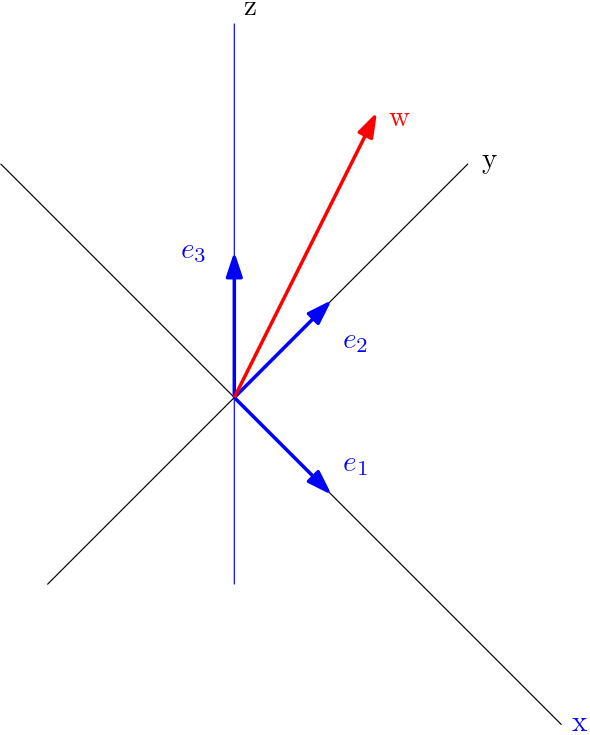
\includegraphics[width=6cm]{vector.png}
    \end{center}

    \begin{equation*}
        w = \begin{bmatrix}
                a \\
                b \\
                c
            \end{bmatrix} = a e_1 + b e_2 + c e_3
    \end{equation*}

    \begin{equation*}
        e_1 = \begin{bmatrix}
                1 \\ 0 \\ 0
            \end{bmatrix}, e_2 = \begin{bmatrix}
                                    0 \\ 1 \\ 0
                                \end{bmatrix}, e_3 = \begin{bmatrix}
                                                        0 \\ 0 \\ 1
                                                    \end{bmatrix}
    \end{equation*}

    \vspace{1em}

    \emph{Examples.}

    \vspace{1em}

    In \(P_3(\mathbb{R})\), let \(P_1 = x^3 + 1, P_2 = x^3 - 2x, P_3 = 4x + 2.\) Is \(P_1, P_2, P_3\) linearly independent?

    To answer the question, we attempt to rpove that they are linearly independent.

    \begin{proof}
        Take arbitrary \(a_1, a_2, a_3 \in \mathbb{R}\). Assume \(a_1 p_1 + a_2 p_2 + a_3 p_3 = 0.\) In other words, \[a_1 (x^3 + 1) + a_2 (x^3 - 2x) + a_3 (4x + 2) = 0 \qquad (1)\] 

        From (1), we can make a system of equations and turn it into a matrix.
        \begin{align*}
            a_1 + a_2    &= 0 \\
            -2a_2 + 4a_3 &= 0 \\
            a_1 + 2 a_3  &= 0
        \end{align*}
        \begin{align*}
            \begin{bmatrix}
                1 & 1  & 0 & 0 \\
                0 & -2 & 4 & 0 \\
                1 & 0  & 2 & 0
            \end{bmatrix} \simeq \begin{bmatrix}
                                    1 & 1  & 0 & 0 \\
                                    0 & -1 & 2 & 0 \\
                                    0 & -1 & 2 & 0 
                                \end{bmatrix} \simeq \begin{bmatrix}
                                    1 & 0 & 2  & 0 \\
                                    0 & 1 & -2 & 0 \\
                                    0 & 0 & 0  & 0
                                \end{bmatrix}
        \end{align*}

        The general solution is \(a_3 = t, a_2 = 2t, a_1 = -2t\). Since we failed to show that \(a_1, a_2, a_3 = 0\), then \(P_1, P_2, P_3\) are linearly dependent. 

        For \(t = 1\), we get \(a_1 = -2, a_2 = 2, a_3 = 1, \) and we find that \(-2P_1 + 2P_2 + 1 P_3 = 0.\)
    \end{proof}

    \subsubsection{Linear Dependence Lemma}

    Suppose \(v_1, \dots, v_m\) is a linearly dependent list in $V$. Then there exists \(j \in \{1,2,\dots,m\}\) such taht the following hold:
    \begin{enumerate}
        \item[(a)] \(v_j \in span(v_1, \dots, v_{j-1});\)
        \item[(b)] if the $j$th term is removed from \(v_1, \dots, v_m\), the span of the remaining list equals \(span(v_1, \dots, v_m)\).   
    \end{enumerate}

    \begin{proof}
        By assumption, \(v_1, \dots, v_m\) are linearly dependent. Therefore, there exist scalars \(a_1, \dots, a_m \in F\) such that \(a_1 v_1 + \dots + a_m v_m = 0\) but not all of \(a_1, \dots, a_m\) are 0.

        Let $j$ be the largest index such that \(a_j \neq 0\). Then \(a_{j+1}, \dots, a_m = 0.\) 

        From our assumption, we have \(a_1 v_1 + \dots + a_j v_j = 0.\) We can write \[a_j v_j = -a_1 v_1 - a_2 v_2 - \dots - a_{j-1} v_{j-1}.\] But since \(a_j \neq 0\), it has a multiplicative inverse. \[v_j = - \frac{a_1}{a_j} v_1 - \frac{a_2}{a_j} v_2 - \dots - \frac{a_{j-1}}{a_j} v_{j-1}.\] This proves (a).

        For (b), note that \[span(v_1, \dots, v_{j-1}, v_{j+1}, \dots, v_m) \subseteq span(v_1, \dots, v_m).\] To show the opposite inclusion, consider some arbitrary \(w \in span(v_1, \dots, v_m).\) We must show \(w \in span(v_1, \dots, v_{j-1}, v_{j+1}, \dots, v_m).\) By assumption, \(w = b_1 v_1 + \dots + b_m v_m\) for such scalars \(b_1, \dots, b_m\). By combining this equation to (a), we get:

        \begin{align*}
            w &= b_1 v_1 + \dots + b_{j-1} v_{j-1} + b_j v_j + b_{j+1} v_{j+1} + \dots + b_m v_m \\
            &= b_1 v_1 + \dots + b_{j-1} v_{j-1} + bj \left( - \frac{a_1}{a_j} v_1 - \frac{a_2}{v_j} v_2 - \dots - \frac{a_{j-1}}{a_j} v_{j-1} \right) \\
            & \qquad + b_{j+1} v_{j+1} + \dots + b_m v_m.
        \end{align*}

        So \(w \in span(v_1, \dots, v_{j-1}, v_{j+1}, \dots, v_m)\) as required.
    \end{proof}

    \subsubsection{Replacement lemma}

    Let $V$ be a finite-dimensional vector space. Consider two lists of vectors:
    \begin{align*}
        u_1, \dots, u_m \qquad & \text{linearly independent in }V \\
        w_1, \dots, w_n \qquad & \text{spans }V
    \end{align*}
    Then we have
    \begin{enumerate}
        \item[(a)] \(m \leq n.\)
        \item[(b)] It is possible to extend the list \(u_1, \dots, u_m\) with \(n-m\) additional vectors from the list \(w_1, \dots, w_n\) such that the resulting list spans $V$.  
    \end{enumerate}

    \begin{proof}
        We shall prove by induction.

        \begin{enumerate}
            \item[(1)] If \(w_1, \dots, w_n\) spans $V$, then \(u_1, w_1, \dots, w_n\) also spans $V$. Also, \(u_1, w_1, \dots, w_n\) is linearly dependent because \(u_1 \in V = span(w_1, \dots, w_n)\), therefore \(u_1\) is a lienar combination of \(w_1, \dots, w_n.\) 
            
            By the linear dependence lemma, one of \(u_1, w_1, \dots, w_n\) can be written as a linear combination of preceding vectors.

            This cannot be \(u_1\) (by linear independence), so some \(w_j\) can be written as a linear combination of preceding vectors.

            By linear dependence lemma part (b), \[span(u_1, w_1, \dots, w_{j-1}, w_{j+1}, \dots, w_n) = V.\]

            \item[(2)] The list of $n$ vectors from (1) spans $V$. Add \(u_2\) to the list: \[u_1, u_2, w_1, \dots, w_{j-1}, w_{j+1}, \dots, w_n.\] Then this list is linearly dependent. One of the $w$'s is redundant and can be removed, without changing the span.
            \item[(3)] Add $u_3$ to the list and it becomes linearly dependent. We remove one of the $w$'s in the list.
            \item[\vdots]
            \item[(m)] Add \(u_m\) to the list and it becomes linearly dependent. We remove one of the $w$'s. Now we have a spanning list of $n$ vectors of the form \[u_1, \dots, u_m,\] followed by $n-m$ of the original $w$'s.
            
            Then \(m \leq n\), because the $n$-vector list starts with \(u_1, \dots, u_m.\) So we have proved (a) and (b).
        \end{enumerate}
    \end{proof}

    \subsubsection{Theorem}

    Every subspace of a finite-dimensional vector space is finite-dimensional.

    \begin{proof}
        Let $V$ be finite-dimensinoal and let $W$ be a subspace of $V$. we must show that $W$ is finite dimensional.
        \begin{enumerate}
            \item[(1)] If \(W = \{0\}\), then $W$ is finite-dimensional and we are done. Otherwise, there exists at least one non-zero vector in $W$. Let \(v_1 \in W\) be such a non-zero vector. Notice that the list of vectors ``\(v_1\)'' is linearly independent.
            \item[(2)] If \(W = span(v_1)\), then $W$ is finite-dimensional and we are done. Otherwise, there exists at least one vector \(v_2 \in W\) such that \(v_2 \notin span(v_1)\). Notice that the list of vectors \(v_1, v_2\) is linearly independent.
            \item[(3)] If \(W = span(v_1,v_2)\), then $W$ is finite-dimensional and we are done. Otherwise, there exists at least one vector \(v_3 \in W\) such that \(v_3 \notin span(v_1,v_2)\). Notice that the list of vectors \(v_1, v_2, v_3\) is linearly independent.
            
            And so on.

            \item[(k)] If \(W = span(v_1, \dots, v_{k-1})\), then $W$ is finite-dimensional and we are done. Otherwise, there exists at least one vector \(v_k \in W\) such that \(v_k \notin span(v_1, \dots, v_{k-1})\). Notice that the list of vectors \(v_1, \dots, v_k\) is linearly independent.  
        \end{enumerate}

        If $W$ were infinite-dimensional, we could repeat this step any number of times, because the ``If'' part would never be done, so in each step, we'd be doing the ``otherwise.''

        This contradicts the assumption that $V$ is finite-dimensional.

        Namely, since $V$ is finite-dimensional, \(V = span(w_1, \dots, w_n)\) is spanned by some finite list of vectors.

        If we repeat the above proceduce \(n+1\) times, we get \(n+1\) linearly independent vectors \(v_1, \dots, v_{n+1}\).

        This contradicts the replacement lemma. Therefore, $W$ is finite-dimensional.
    \end{proof}

    \pagebreak


    \section{2.B Bases}

    \subsection{Bases}

    \subsubsection{Definition}

    A \emph{basis} of $V$ is a list of vectors in $V$ that is linearly independent and spans $V$.

    \subsubsection{Examples}

    \begin{enumerate}
        \item[(a)] \begin{equation*}
                        \begin{bmatrix}
                            1 \\ 0 \\ 0
                        \end{bmatrix}, \begin{bmatrix}
                                            0 \\ 1 \\ 0
                                        \end{bmatrix}, \begin{bmatrix}
                                                            0 \\ 0 \\ 1
                                                        \end{bmatrix} \text{ is a basis of } \mathbb{R}^3.
                   \end{equation*} 
        \item[(b)] \begin{equation*}
            \begin{bmatrix}
                1 \\ 3 \\ 5
            \end{bmatrix}, \begin{bmatrix}
                                0 \\ 1 \\ 2
                            \end{bmatrix}, \begin{bmatrix}
                                                1 \\ 1 \\ 5
                                            \end{bmatrix} \text{ is a basis of } \mathbb{R}^3
        \end{equation*}
        \item[(c)] \[ 1, x, x^2, x^3 \text{ is a basis of } \mathcal{P}_3(\textbf{F}) \]
    \end{enumerate}

    \subsubsection{Criterion for basis}

    A list \(v_1, \dots, v_n\) of vectors in $V$ is a basis of $V$ if and only if every \(v \in V\) can be written uniquely in the form \[v = a_1 v_1 + \dots + a_n v_n,\] where \(a_1, \dots, a_n \in \textbf{F}.\)

    \begin{proof}
        Suppose \(v_1, \dots, v_n\) is a basis of $V$. Let \(v \in V\). Since \(v_1, \dots, v_n\) spans $V$, there exists \(a_1, \dots, a_n \in \textbf{F}\) such that \[v = a_1 v_1 + \dots  a_n v_n.\] To show that it is unique, suppose that \(c_1, \dots, c_n\) are scalars where \(v = c_1 v_1 + \dots + c_n v_n\). Subtracting this equation from the previous, we get \[0 = (a_1 - c_1) v_1 + \dots + (a_n - c_n)v_n.\] This completes the proof for uniqueness.

        In the other direction, suppose every \(v \in V\) can be written uniquely in the form \[v = a_1 v_1 + \dots + a_n v_n.\] This implies that \(v_1, \dots, v_n\) spans $V$. To show that \(v_1, \dots, v_n\) are linearly independent, suppose that \(a_1, \dots, a_n \in \textbf{F}\). Then \[0 = a_1 v_1 + \dots + a_n v_n.\] Thus \(v_1, \dots, v_n\) is linearly independent and hence is a basis of $V$.
    \end{proof}

    \subsection{Coordinates}

    If \(B = v_1, \dots, v_n\) is a basis of $V$, and \(v = a_1 v_1 + \dots + a_n v_n\), then we say \(a_1, \dots, a_n\) are the \emph{coordinates} of $v$ with respect to the basis $B$.

    \subsubsection{Examples of coordinates}

    Suppose that \(B = 1,x,x^2, x^3\) is the basis of \(\mathcal{P}_3 (\mathbb{R})\). Find the coordinates of \(p = (1+2x)(3x + x^2)\) with respect to the basis $B$.

    \vspace{1em}

    \textbf{Solution:}
    \begin{align*}
        p &= (1 + 2x)(3x + x^2) \\
          &= 3x + x^2 + 6x^2 + 2x^3 \\
          &= 3x + 7x^2 + 2x^3 \\
          &= 0 \cdot 1 + 3 \cdot x + 7 \cdot x^2 + 2 \cdot x^3
    \end{align*}
    The coordinates are: 0, 3, 7, and 2.

    \vspace{1em}

    Another basis for \(\mathcal{P}_3(\mathbb{R})\) is \(B' = 1, (x-1), (x-1)^2, (x-1)^3\). Find the coordinates of \(p = 3x + 6x^2 + 2x^3\) in the basis $B'$.

    \vspace{1em}

    \textbf{Solution:} Suppose that \(y = x - 1\) and \(x = y + 1\). Then 
    \begin{align*}
        p &= 3(y+1) + 7(y + 1)^2 + 2(y+1)^3 \\
          &= 3y + 3 + 7y^2 + 14y + 7 + 2y^3 + 6y^2 + 6y + 2 \\
          &= 12 + 23y + 13 y^2 + 2y^3 \\
          &= 12 + 23(x-1) + 13(x-1)^2 + 2(x-1)^3
    \end{align*}
    The coordinates of $p$ with respect to $B'$ are: 12, 23, 13, and 2.

    \subsection{Theorems about Bases}

    \subsubsection{Spanning list contains a basis}

    Every spanning list in a vector space can be reduced to a basis of the vector space (by removing 0 or more vectors from the list).

    \begin{proof}
        Suppose \(v_1, \dots, v_n\) spans $V$. We want to remove some of the vectors from \( v_1, \dots, v_n \) so that the remaining vectors form a basis of $V$. We do this through induction.

        Start with $B$ equal to the list \(v_1, \dots, v_n.\)

        \begin{enumerate}
            \item[\textbf{Step 1}] If \(v_1 = 0\), delete \(v_1\) from $B$. If \(v_1 \neq 0\), leave $B$ unchanged.
            \item[\textbf{Step $j$}] If \(v_j\) is in \(span(v_1, \dots, v_{j-1})\), delete \(v_j\) from $B$. If \(v_j\) is not in \(span(v_1, \dots, v_{j-1})\), leave $B$ unchanged.  
        \end{enumerate}

        Stop the process after step $n$, getting a list $B$. This list spans $V$ because our original list spanned $V$ and we have discarded vectors that were already in the span of the previous vectors. This process ensures that no vector in $B$ is in the span of the previous ones. Thus, $B$ is linearly independent, by the Linear Dependence Lemma. Hence $B$ is a basis of $V$.
    \end{proof}

    \subsubsection{Basis of finite-dimensional vector space}

    Every finite-dimensional vector space has a basis.

    \begin{proof}
        By definition, a finite-dimensional vector space has a spanning list. The previous result tells us that each spanning list can be reduced to a basis.
    \end{proof}

    \subsubsection{Linearly independent list extends to a basis}

    Every linearly indepdendent list of vectors in a finite-dimensional vector space can be extended to a basis of the vector space.

    \begin{proof}
        Suppose \(u_1, \dots, u_m\) is linearly independent in a finite-dimensional vector space $V$. Let \(w_1, \dots, w_n\) be a basis of $V$. Thus the list \[u_1, \dots, u_m, w_1, \dots, w_n\] spans $V$. Applying the produce of the proof of 3.1 to reduce this list to a basis of $V$ produces a basis consisting of the vectors \(u_1, \dots, u_m\) (none of the $u$'s get deleted because \(u_1, \dots, u_m\) is linearly independent) and some of the $w$'s.
    \end{proof}

    \subsubsection{Every subspace of $V$ is part of a direct sum equal to $V$}

    Suppose $V$ is finite-dimensional and $U$ is a subspace of $V$. Then there is a subspace $W$ of $V$ such that \(V = U \oplus W\).

    \begin{proof}
        Since $V$ is finite-dimensional, so is $U$. Thus, there is a basis \(u_1, \dots, u_m\) of $U$ and is linearly independent in $V$. Hence, this list can be extended to a basis \(u_1, \dots, u_m, w_1, \dots, w_n\) of $V$. Let \(W = span(w_1, \dots, w_n)\).
        
        \vspace{1em}

        To prove that \(V = U \oplus W\), we need to show that \[V = U + W \text{ and } U \cap W = \{0\}.\]

        Proving the first equation, suppose \(v \in V\) Then, since the list \(u_1, \dots, u_m, w_1, \dots, w_n\) spans $V$, there exist \(a_1, \dots, a_m, b_1, \dots, b_n \in \textbf{F}\) such that 
        \begin{equation*}
            v = \underbrace{a_1u_1 + \dots + a_m u_m}_{u} + \underbrace{b_1 w_1 + \dots + b_n w_n}_{w} \Rightarrow v = u + w, u \in U, w \in W.
        \end{equation*}
        Thus we have \(v \in U + W\).

        Proving the second equation, suppose \(v \in U \cap W\). There exists scalars \(a_1, \dots, a_m, b_1, \dots, b_n \in \textbf{F}\) such that \[ v = a_1 u_1 + \dots + a_m u_m = b_1 w_1 + \dots + b_n w_n. \] Thus \[a_1 u_1 = \dots + a_m u_m - b_1 w_1 - \dots - b_n w_n = 0.\] Since \(u_1, \dots, u_m, w_1, \dots, w_n\) is linearly independent, this implies \(a_1 = \dots = a_m = b_1 = \dots = b_n = 0.\) Thus \(v = 0\) and this completes the proof.
    \end{proof}

    \pagebreak

    \section{2.C Dimension}

    \subsection{Basis length does not depend on basis}

    Any two bases of a finite-dimensional vector space have the same length.

    \begin{proof}
        Suppose $V$ is finite-dimensional. Let $B_1$ and $B_2$ be two bases of $V$. Then $B_1$ is linearly independent in $V$ and $B_2$ spans $V$, so the length of $B_1$ is at most length of $B_2$. Interchanging the roles, we also see that the length of $B_2$ is at most the length of $B_1$. Thus the length of $B_1$ equals the length of $B_2$, as desired.
    \end{proof}

    \subsection{Definition of a dimension}

    \begin{itemize}
        \item The \emph{dimension} of a finite-dimensional vector space is the length of any basis of the vector space.
        \item The dimension of $V$ (if $V$ is finite-dimensional) is denoted by \(\dim V\).
    \end{itemize}

    \subsection{Examples of a dimension}

    \begin{enumerate}
        \item \(\dim \textbf{F}^n = n\) because the standard basis of \(\textbf{F}^n\) has length $n$.
        \item \(\dim \mathcal{P}_m(\textbf{F}) = m + 1\) because the basis \(1,z,\dots,z^m\) of \(\mathcal{P}_m(\textbf{F})\) has length $m$ + 1.
    \end{enumerate}

    \subsection{Dimension of a subspace}

    If $V$ is finite-dimensional and $U$ is a subspace of $V$, then \(\dim U \leq \dim V.\)

    \begin{proof}
        Suppose $V$ is finite-dimensional and $U$ is a subspace of $V$. Think of a basis of $U$ as a linearly independent list in $V$, and think of a basis of $V$ as a spanning list in $V$. These linearly independent vectors \(u_1, \dots, u_m\) can be extended to a basis of $V$. That extended basis has at least $m$ vectors, so \(\dim V \geq \dim U.\)
    \end{proof}

    \subsection{Linearly independent list of the right length is a basis}

    Suppose $V$ is finite-dimensional. Then every linearly independent list of vectors in $V$ with length \(\dim V\) is a basis of $V$.

    \begin{proof}
        Suppose \(\dim V = n\) and \(v_1, \dots, v_n\) is linearly independent in $V$. The list \(v_1, \dots, v_n\) can be extended to a basis of $V$. However, every basis of $V$ has length $n$, so in this case the extension is the trivial one, meaning that no elements are adjoined to \(v_1, \dots, v_n\). In other words, \(v_1, \dots, v_n\) is a basis of $V$, as desired.
    \end{proof}

    \subsection{Examples}

    \begin{enumerate}
        \item Show that the list \((5,7), (4,3)\) is a basis of \(\textbf{F}^2\). 
        \begin{proof}
            The two vectors are linearly independent (because neither vector is a scalar multiple of the other). Note that \(\textbf{F}^2\) has dimension 2. Thus, Theorem 1.5 implies that the linearly independent list of length 2 is a basis of \(\textbf{F}^2\).
        \end{proof}
        \item Show that \(p(x) = x^2 + 1, q(x) = x^2 + x, r(x) = x^2\) are a basis of \(\mathcal{P}_2(\textbf{F})\).
        \begin{proof}
            Assume \(a(x^2 + 1) + b(x^2 + x) + c(x^2) = 0\), where \(a,b,c \in \textbf{F}\). Then we have \((a + b + c)x^2 + bx + a = 0 \Rightarrow a + b + c = 0.\) We know that \(a = b = 0\) so it follows that \(c = 0\). Hence, $p,q,r$ are linearly independent. Since we know that \(\dim \mathcal{P}_2(\textbf{F}) = 3\) then by Theorem 1.5, $p,q,r$ are bases of \(\mathcal{P}_2(\textbf{F})\).
        \end{proof}
    \end{enumerate}

    \subsection{Spanning list of the right length is a basis}

    Suppose $V$ is finite-dimensional. Then every spanning list of vectors in $V$ with length \(\dim V\) is a basis of $V$.

    \begin{proof}
        Suppose \(\dim V = n\) and \(v_1, \dots, v_n\) spans $V$. The list \(v_1, \dots, v_n\) can be reduced to a basis of $V$ (by removing 0 or more vectors from the list). However, every basis of $V$ has length $n$, so the reduction is the trivial one, meaning that no elements are deleted from \(v_1, \dots, v_n\). In other words, \(v_1, \dots, v_n\) is a basis of $V$, as desired.
    \end{proof}

    \subsection{Dimension of a sum}

    If $U_1$ and $U_2$ are subspaces of a finite-dimensional vector space, then \[\dim(U_1 + U_2) = \dim U_1 + \dim U_2 - \dim(U_1 \cap U_2).\]

    \begin{proof}
        Let \(u_1, \dots, u_m\) be a basis of \(U_1 \cap U_2\); thus \(\dim (U_1 \cap U_2) = m\). These basis are linearly independent in $U_1$ and can be extended to a basis \(u_1, \dots, u_m, v_1, \dots, v_j\). Thus, \(\dim U_1 = m + j\) Also, \(u_1, \dots, u_m, w_1, \dots, w_k\) of $U_2$ and so \(\dim U_2 = m + k\).

        We need to show that \(u_1, \dots, u_m, v_1, \dots, v_j, w_1, \dots, w_k\) is a basis of \(U_1 + U_2\). so
        \begin{align*}
            \dim(U_1 + U_2) &= m + j + k \\
                            &= (m+j) + (m+k) - m \\
                            &= \dim U_1 + \dim U_2 - \dim (U_1 \cap U_2).
        \end{align*}
        Clearly \(span(u_1,\dots,u_m,v_1,\dots,v_j,w_1, \dots, w_k)\) contains \(U_1 + U_2\) which equals \(U_1 + U_2\). To show that this list is a basis of \(U_1 + U_2\), we need to show that it is linearly independent. Suppose that \[a_1 u_1 + \dots + a_m u_m + b_1 v_1 + \dots + b_j v_j + c_1 w_1 + \dots + c_k w_k = 0\] where \(a,b,c \in \textbf{F}\). Then \[c_1 w_1 + \dots + c_k w_k = -a_1 u_1 - \dots - a_m u_m - b_1 v_1 - \dots - b_j v_j.\] This implies that \(c_1 w_1 + \dots + c_k w_k \in U_1\) and consequently, \(c_1 w_1 + \dots + c_k w_k \in U_1 \cap U_2\). Since \(u_1, \dots, u_m\) is a basis of \(U_1 \cap U_2\), we can write \[c_1 w_1 + \dots + c_k w_k = d_1 u_1 + \dots + d_m u_m\] for some scalars \(d \in \textbf{F}\). But \(u_1, \dots, u_m, w_1, \dots, w_k\) are linearly independent, so all $c$'s and $d$'s equal 0. Thus, our original equation becomes \[ a_1 u_1 + \dots + a_m u_m + b_1 v_1 + \dots + b_j v_j = 0. \] Since \(u_1, \dots, u_m, v_1, \dots, v_j\) are linearly independent, then all $a$'s and $b$'s equal 0. 
    \end{proof}

\end{document}